\section{Vorbereitungsfragen}
\subsection{Begriffsdefinitionen}

\begin{itemize}
\item \textbf{Wärmedurchgang} ist der Wärmeübergang von einem Fluid durch eine Wand auf ein anderes Fluid und wird durch den Wärmedurchgangskoeffizienten beschrieben. Der Wärmedurchgangskoeffizient ist ein stoffspezifischer Wert und wird nach \autoref{eq:230523_Wärmedurchgangskoeff} berechnet. 
 
\begin{equation}
	\centering
	u=\frac{1}{R_{si}+\sum_{i=1}^N \frac{d_i}{\lambda_i}+R_{se}}
	\label{eq:230523_Wärmedurchgangskoeff}
\end{equation}

\item Der \textbf{Wärmeübergangswiderstand} $R_s$ beschreibt die Wärmeübertragung zwischen einem Festkörper und einem Fluid. Er ist als der Kehrwert des Wärmeübergangskoeffizienten definiert.

\item Die \textbf{Wärmeleitfähigkeit} $\lambda$ ist die Stoffeigenschaft eines Materials einen Wärmestrom zu leiten. Sie gibt Aussage darüber wie sich Wärme in einem Stoff ausbreitet und ist auch stoffspezifisch.

\item \textbf{Wärmestrahlung} ist eine Art der Wärmeübertragung durch elektromagnetische Wellen im infraroten Bereich.

\end{itemize}


\subsection{Temperaturverlauf und Wärmestrom durch ein- und mehrschichtige Wände}
\begin{figure}[H]
	\centering
	\begin{subfigure}[c]{0.303\textwidth}
		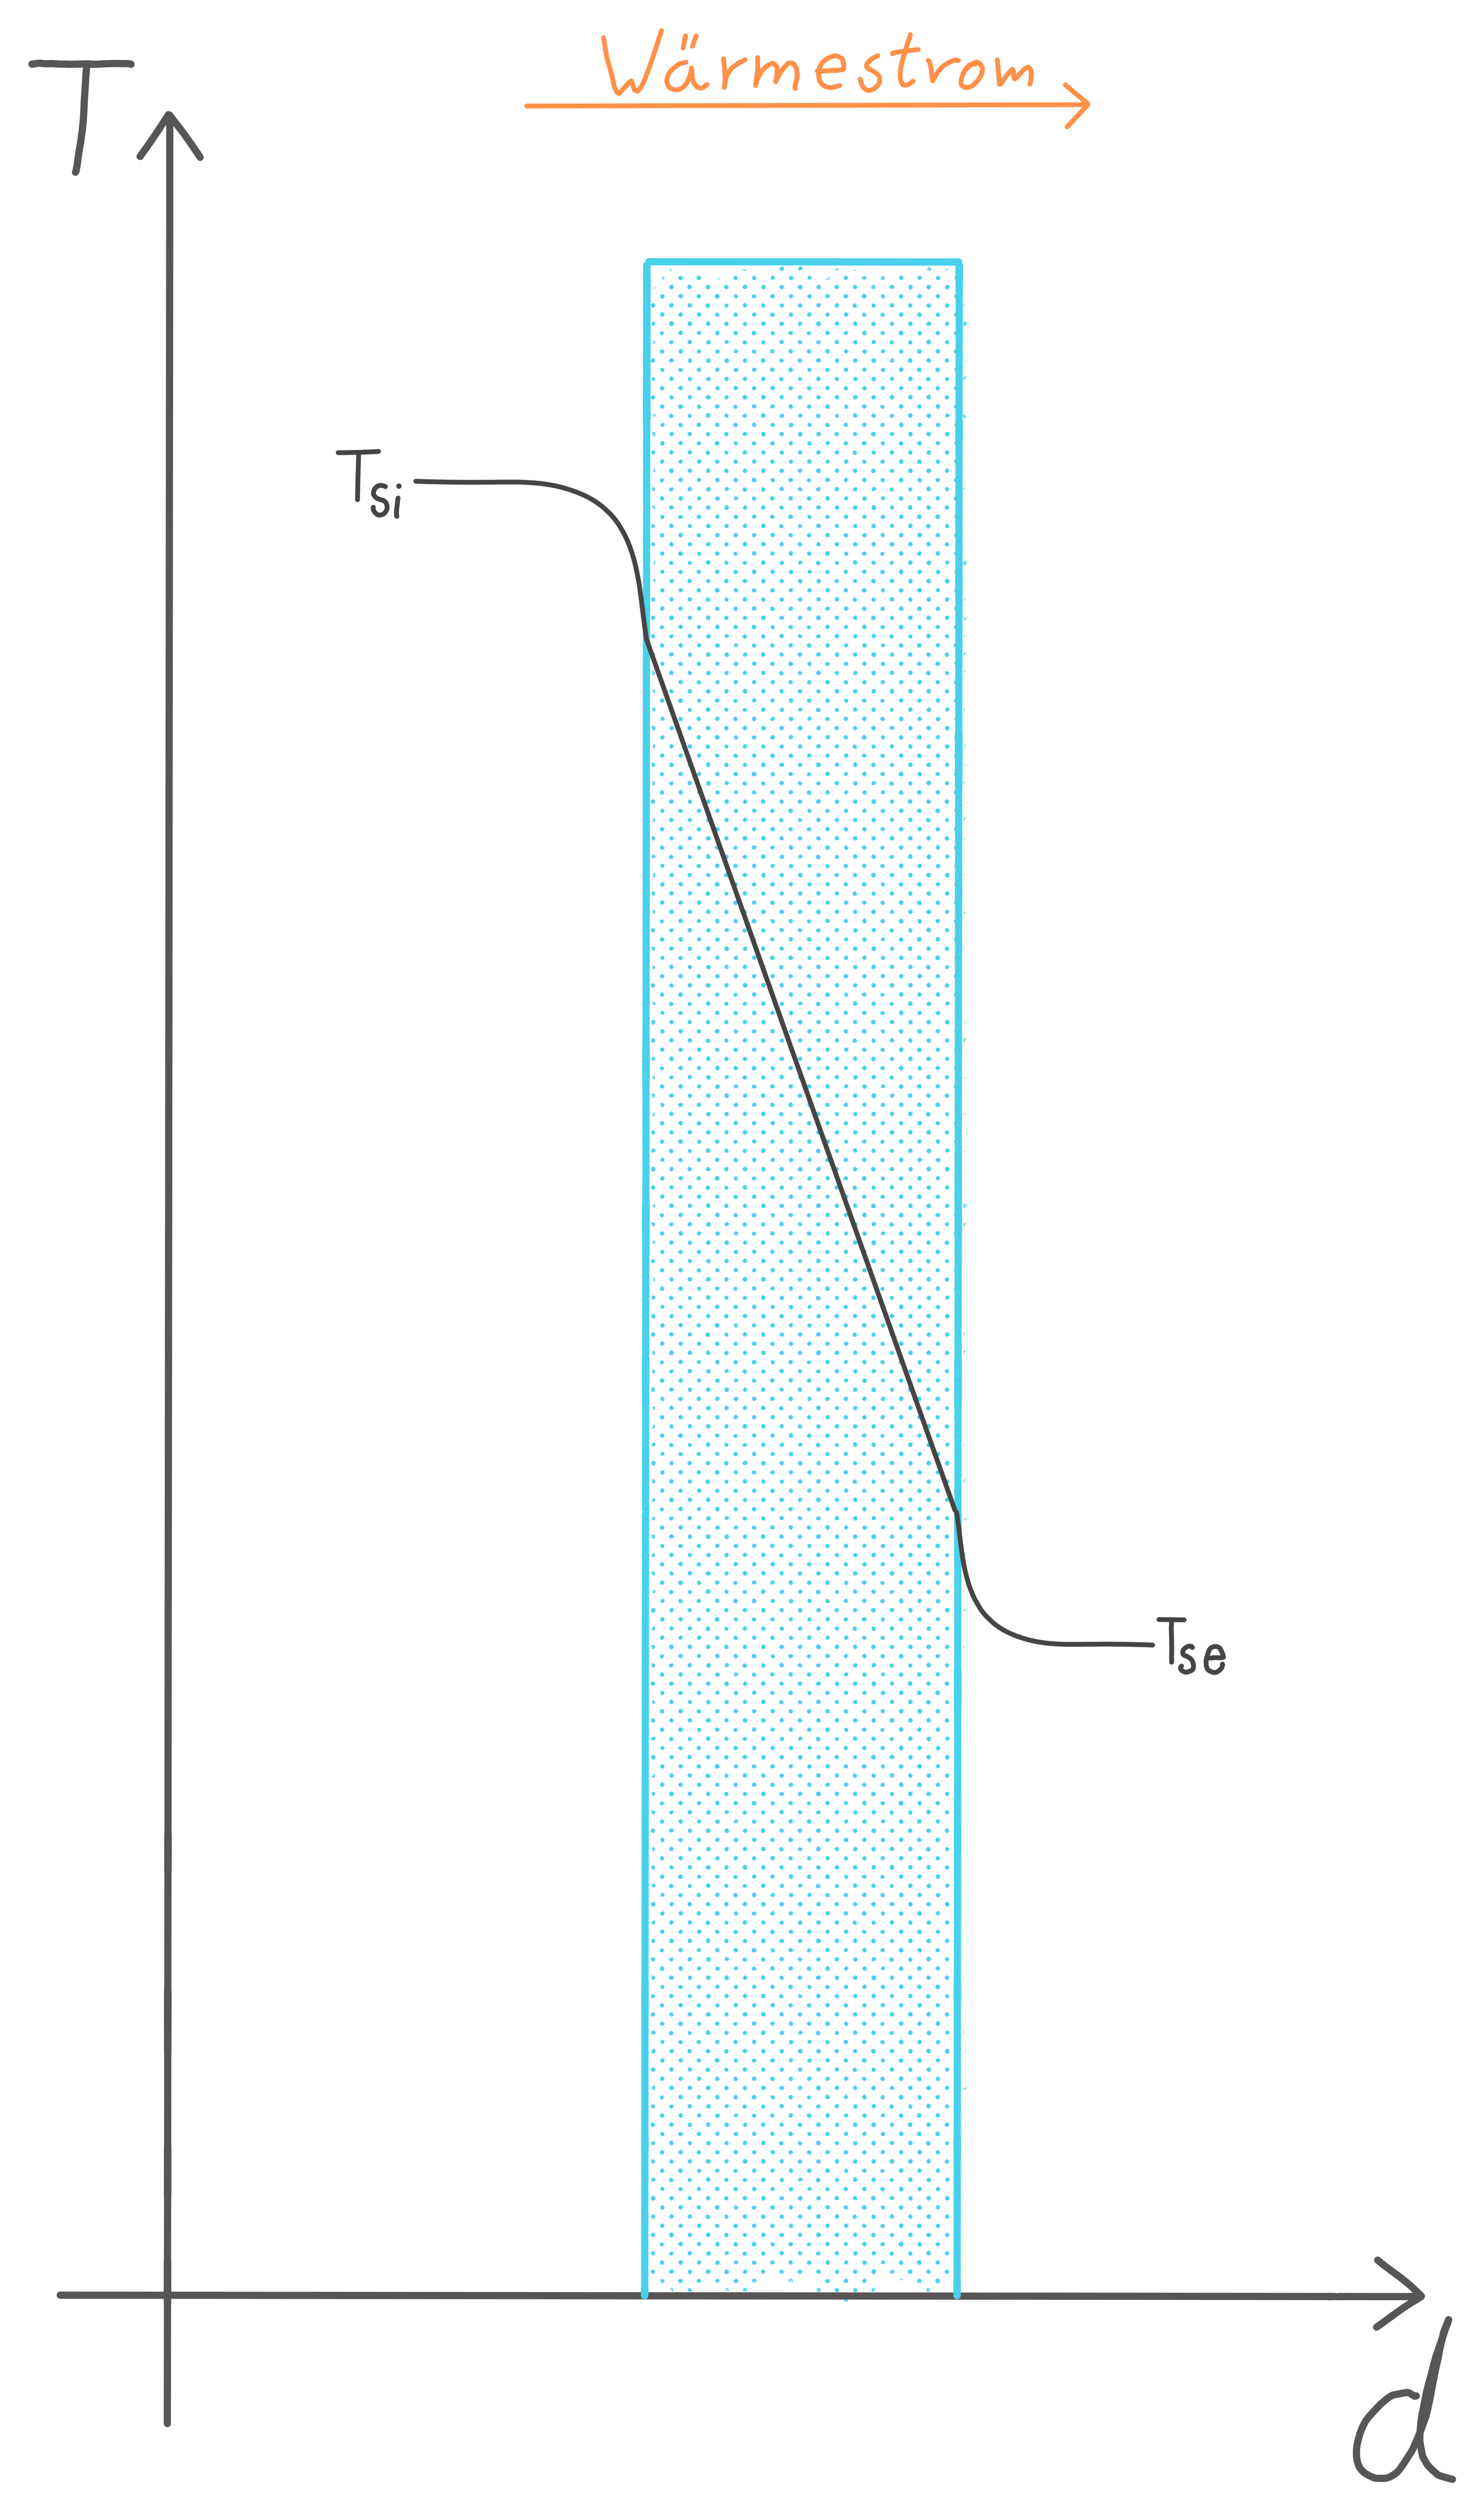
\includegraphics[width=\textwidth]{Abbildungen/einschichtig.png}
		\caption{Einschichtige Wand}
	\end{subfigure}
	\begin{subfigure}[c]{0.497\textwidth}
		\includegraphics[width=\textwidth]{Abbildungen/mehrschichtig.png}
		\caption{Mehrschichtige Wand}
	\end{subfigure}
	\caption{Skizzen der Temperaturverläufe und Wärmeströme verschiedener Wände}
	\label{fig:230515_Temp-verlauf}
\end{figure}

\subsection{Wärmedurchgangskoeffizient}
Der Wärmedurchgangskoeffizient U ist eine Kennzahl, die den Wärmedurchgang durch einen Bauteil oder eine Bauteilschicht beschreibt. 
Er gibt an, wie viel Wärme pro Zeiteinheit und pro Fläche durch das Bauteil hindurchgeht, wenn ein Temperaturunterschied zwischen den beiden Seiten des Bauteils herrscht.
Der U-Wert wird in der Einheit $$\frac{W}{m^2 \cdot K}$$ angegeben. Je niedriger der U-Wert, desto besser ist die Wärmedämmung des Bauteils. 
Ein niedriger U-Wert bedeutet, dass weniger Wärmeenergie verloren geht und das Bauteil effizienter dämmt.
Der U-Wert berücksichtigt verschiedene Faktoren wie die Materialien, die Dicke der Bauteilschichten, eventuelle Luftspalten und Wärmebrücken. 
Er wird verwendet, um den Energieverbrauch von Gebäuden zu berechnen, die Effizienz von Wärmedämmmaßnahmen zu bewerten und den Wärmeschutz von Bauteilen zu beurteilen.

\subsection{Reduzierung der Auswirkungen von Temperaturschwankungen}

Die physikalisch simpelste Lösung, um Temperaturschwankungen von Außen nach Innen entgegenzuwirken, ist es die Wand massiver zu machen, wodurch die Trägheit des Systems erhöht wird.
Bei einer hohen Trägheit verhält sich das System wie ein Tiefpassfilter, langsame Temperaturschwankungen sind auf der Innenseite jedoch immernoch merkbar.
Die bessere Lösung ist es, die Wandkomposition zu verändern und eine bessere Dämmung einzubauen.
Das kann durch mehrere Schichten und/oder interne Luftschichten erzielt werden.
Dies hat den Effekt, dass die Innentemperaturen besser gehalten und leichter geregelt werden können.

\subsection{Gesamtwärmedurchgangswiderstand in mehrschichtigen Wänden}
\begin{equation}
	\label{eq:130723_Wärmedurchgangswiderstand}
	R_{tot}=R_{si}+\sum_{i=1}^N \frac{d_i}{\lambda_i}+R_{se}
\end{equation}

Die grundlegende Gleichung zur Berechnung von $R_{tot}$ ist \autoref{eq:130723_Wärmedurchgangswiderstand} wobei $R_{si}=0,13\frac{m^2 \cdot K}{W}$ und $R_{se}=0,04\frac{m^2 \cdot K}{W}$  gegebene Werte sind.
Für die weitere Berechnung werden für die $\lambda$-Werte der Baustoffe immer die jeweils höchsten Werte angenommen (siehe Excel-Datei). Aus den entsprechenden Normen werden
die $\lambda$-Werte für Holz \cite[S.20]{lamda-holz-luft} $\lambda_{Holz}=0,24\frac{W}{m\cdot K}$ und Luft\cite[S. 15]{lamda-holz-luft} $\lambda_{Luft}=0,25\frac{W}{m\cdot K}$ abgelesen. (DIN EN ISO 10456:2010-05)
Der $\lambda$-Wert für XPS \cite[S.23]{lamda-xps} beträgt $\lambda_{XPS}=0,046\frac{W}{m\cdot K}$ (DIN 4108-4:2020-11). Daraus ergibt sich folgende Rechnung:

$$R_{tot}=0,13 \frac{m^2 \cdot K}{W}+ \frac{0,016m}{0,046 \frac{W}{m \cdot K}}+\frac{0,0224}{0,24 \frac{W}{m \cdot K}} +0,04 \frac{m^2 \cdot K}{W}$$

$$R_{tot}=0,61\frac{m^2 \cdot K}{W}$$
Der U-Wert ergibt sich aus dem Kehrwert des Wärmedurchgangswiderstands und beträgt:
$$U_{Wand 1}=1,6362 \frac{W}{m^2 \cdot K}$$

$$R_{tot}=0,13\frac{m^2 \cdot K}{W}+ \frac{0,006m}{0,046\frac{W}{m\cdot K}}+ \frac{0,01}{0,025\frac{W}{m\cdot K}} +\frac{0,0122}{0,24\frac{W}{m\cdot K}} +0,04\frac{m^2 \cdot K}{W}$$
Für die zweite Wand beträgt der Widerstand:
$$R_{tot}=0,75\frac{m^2 \cdot K}{W}$$
Analog zum vorherigen Wandaufbau beträgt der U-Wert:
$$U_{Wand 2}=1,3311 \frac{W}{m^2 \cdot K}$$



\subsection{Unterschiede zwischen Norm und berechneten U-Werten}
Für die Normierung von Werten werden über lange Zeiträume Messungen erstellt und ein Normwert gebildet.
Der Versuch stellt in diesem Zeitrahmen nur eine Einzelmessung dar. 
Innerhalb der Architektur von Gebäuden kommt es zu unterschiedlichen U-Werten durch bauliche Unterschiede.
In den oberen Stockwerken führt die Luftzirkulation und damit einhergehende Konvektion zu einem anderen U-Wert als im Kellergeschoss, wo die angrenzende Erdschicht Einfluss nimmt.
Andere klimatische Rahmenbedingungen können dazu führen, dass sich U-Werte regional unterscheiden. 
